% Chapter 2

\chapter{Quantum Operations} % Main chapter title

\label{Chapter2}

\section{Rotations}
\label{chapter:rotation}

To replicate the functionality of a computational neuron, the behavior of a qubit in combination with different gates is observed. All gates rotate the state of the qubit in the Bloch sphere. Due to this one cannot fully replicate the core functionality of a computational neuron, as the gate operations are of additive nature to the initial state of the qubit. The following figures \ref{fig:circuit_empty} to \ref{fig:histogram_ry} demonstrate the behavior single gates have on the qubit state through the Bloch sphere.

\todo{Explain all gates, what does it and where is it used and why}

\begin{figure}[!h]
    \centering
    \scalebox{1.0}{
        \Qcircuit @C=1.0em @R=1.0em @!R { 
            \nghost{ {q}_{0} :  } & \lstick{ {q}_{0} :  } & \qw & \qw\\ 
        }
    }
    \caption{Empty single qubit circuit}
    \label{fig:circuit_empty}
\end{figure}

\begin{figure}[!h]
    \centering
    \scalebox{0.3}{
        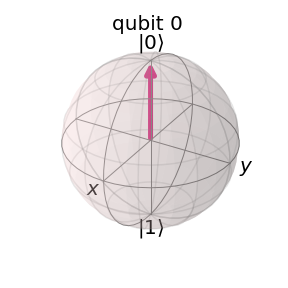
\includegraphics{Appendices/chapter_2/basic_bloch_sphere.png}
    }
    \caption{State vector on bloch sphere}
    \label{fig:circuit_empty_bloch_sphere}
\end{figure}

\begin{figure}[!h]
    \centering
    \scalebox{1.0}{
        \Qcircuit @C=1.0em @R=1.0em @!R { 
            \nghost{ {q}_{0} :  } & \lstick{ {q}_{0} :  } & \gate{\mathrm{X}} & \qw & \qw\\ 
        }
    }
    \caption{Negated single qubit circuit}
    \label{fig:circuit_negated_empty}
\end{figure}

\begin{figure}[!h]
    \centering
    \scalebox{0.3}{
        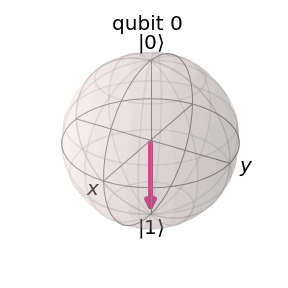
\includegraphics{Appendices/chapter_2/negated_bloch_sphere.png}
    }
    \caption{Negated state vector on bloch sphere}
    \label{fig:circuit_negated_empty_bloch_sphere}
\end{figure}

\newpage

\begin{figure}
    \centering
    $\mathrm{X} = \begin{pmatrix}
        0 & 1 \\
        1 & 0
    \end{pmatrix}$
    \caption{Pauli X gate matrix}
    \label{fig:matrix_pauli_x}
\end{figure}

Figure \ref{fig:circuit_empty_bloch_sphere} and \ref{fig:circuit_negated_empty_bloch_sphere} show that a rotation with an $X$ gate inverst the state from $\ket{0}$ to $\ket{1}$ and vice versa. The matrix behind the $X$ gate\cite{qiskit_xgate_nodate} is shown in figure \ref{fig:matrix_pauli_x} and an example calculated in equation \ref{equation:pauli_x_example}.

\begin{equation}
    \centering
    \begin{split}
        \mathrm{X}\ket{0} =\ \begin{pmatrix} 0 & 1 \\ 1 & 0 \end{pmatrix}\begin{pmatrix}1 \\ 0\end{pmatrix} =\ \begin{pmatrix}0 \\ 1\end{pmatrix} =\ \ket{1}
    \end{split}
    \label{equation:pauli_x_example}
\end{equation}

Using the Hadamard\cite{qiskit_hgate_nodate} gate defined in figure \ref{fig:matrix_hadamard}, a single qubit can be put into a superposition, where both $\ket{0}$ and $\ket{1}$ have the same probability. This is shown in equation \ref{equation:hadamard_example}. The visualization done using the circuit \ref{fig:circuit_hadamard} in figure \ref{fig:circuit_hadamard_bloch_sphere} demonstrates that the state vector is set orthogonal to the $Z$ axis.

\begin{figure}[!h]
    \centering
    $\mathrm{H} = \frac{1}{\sqrt{2}}\begin{pmatrix}1 & 1 \\1 & -1\end{pmatrix}$
    \caption{Hadamard gate matrix}
    \label{fig:matrix_hadamard}
\end{figure}

\begin{equation}
    \centering
    \begin{split}
        \mathrm{H}\ket{0} =\ \frac{1}{\sqrt{2}}\begin{pmatrix}1 & 1 \\1 & -1\end{pmatrix}\begin{pmatrix}1 \\ 0\end{pmatrix} =\ \frac{\ket{0} + \ket{1}}{\sqrt{2}}
    \end{split}
    \label{equation:hadamard_example}
\end{equation}


\begin{figure}[!h]
    \centering
    \scalebox{1.0}{
        \Qcircuit @C=1.0em @R=1.0em @!R { 
            \nghost{ {q}_{0} :  } & \lstick{ {q}_{0} :  } & \gate{\mathrm{H}} & \qw & \qw\\ 
        }
    }
    \caption{Circuit with Hadamard gate}
    \label{fig:circuit_hadamard}
\end{figure}

\begin{figure}[!h]
    \centering
    \scalebox{0.3}{
        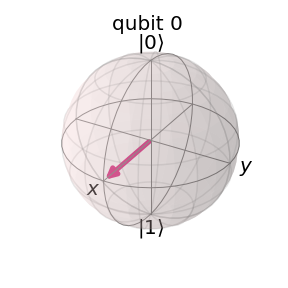
\includegraphics{Appendices/chapter_2/hadamard_bloch_sphere.png}
    }
    \caption{Superposition state on bloch sphere}
    \label{fig:circuit_hadamard_bloch_sphere}
\end{figure}


As discussed in chapter \ref{chapter:quantum_embedding}, there are multiple ways of encoding values onto qubits. The parameterizable gates allow the rotation around a defined axis for the given value, where the value of $\pi$ equals one $180°$ rotation, and $2\pi$ a full $360°$ rotation. One of these gates is the $\mathrm{RY}$ gate\cite{qiskit_rygate_nodate}. Its matrix \ref{fig:matrix_ry} has the parameter $\theta$ which is substituted with any given value. Its functionality is measured and displayed in histogram \ref{fig:histogram_ry}, which uses the circuit \ref{fig:circuit_ry} and $\theta =\ \frac{\pi}{2}$ to create a superposition (\ref{fig:ry_bloch_sphere}) \emph{comparable}\footnote{Not completely equal, as the global phase is not the same as when using the Hadamard gate} to the one seen in figure \ref{fig:circuit_hadamard_bloch_sphere}.

\clearpage

\todo{Explain why $cos$, $sin$ on first occurence, also for other gates. Why is this gate used}


\begin{figure}[!h]
    \centering
    $$
    \mathrm{RY}(\theta) = exp(-i \frac{\theta}{2} Y) =
    \begin{pmatrix}
        \cos{\frac{\theta}{2}} & -\sin{\frac{\theta}{2}} \\
        \sin{\frac{\theta}{2}} & \cos{\frac{\theta}{2}}
    \end{pmatrix}
    $$
    \caption{RY gate matrix}
    \label{fig:matrix_ry}
\end{figure}

\begin{figure}[!h]
    \centering
    \scalebox{1.0}{
        \Qcircuit @C=1.0em @R=1.0em @!R { 
            \nghost{ {q}_{0} :  } & \lstick{ {q}_{0} :  } & \gate{\mathrm{R_Y}\,(\frac{\pi}{2})} & \qw & \qw\\ 
        }
    }
    \caption{Circuit with RY gate parameterized to $\frac{\pi}{2}$}
    \label{fig:circuit_ry}
\end{figure}

\begin{figure}[!h]
    \centering
    \scalebox{0.3}{
        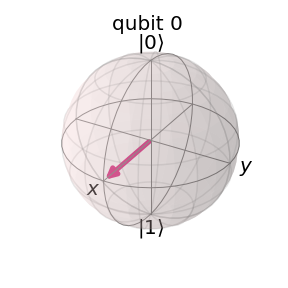
\includegraphics{Appendices/chapter_2/halfpi_yrotation_bloch_sphere.png}
    }
    \caption{Superposition state on bloch sphere using RY gate}
    \label{fig:ry_bloch_sphere}
\end{figure}

\begin{figure}[!h]
    \centering
    \scalebox{0.5}{
        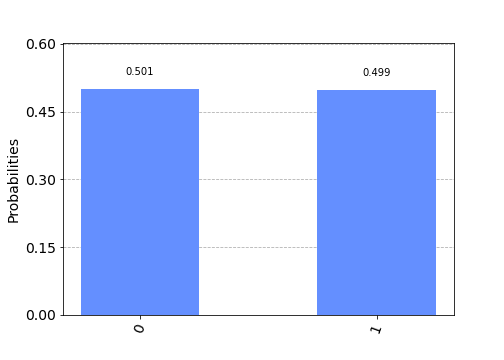
\includegraphics{Appendices/chapter_2/halfpi_yrotation_histogram.png}
    }
    \caption{Histogram of measurments done on circuit \ref{fig:circuit_ry}}
    \label{fig:histogram_ry}
\end{figure}

When explaining the behavior of more complex gates that involve more than one qubit we have to dismiss the visualization with the Bloch sphere and move to using the final state vector $\vec{s}$, which can accurately show the resulting probabilities for all states. Figure \ref{fig:circuit_double_hadamard} shows two qubits that pass through Hadamard gates, and equation \ref{equation:two_hadamard_example} shows the state vector.

\begin{figure}[!h]
    \centering
    \scalebox{1.0}{
        \Qcircuit @C=1.0em @R=1.0em @!R { 
            \nghost{ {q}_{0} :  } & \lstick{ {q}_{0} :  } & \gate{\mathrm{H}} & \qw & \qw\\ 
            \nghost{ {q}_{1} :  } & \lstick{ {q}_{1} :  } & \gate{\mathrm{H}} & \qw & \qw\\ 
        }
    }
    \caption{Circuit with two Hadamard gates}
    \label{fig:circuit_double_hadamard}
\end{figure}

\begin{equation}
    \centering
    \begin{split}
        \mathrm{H}\ket{0} &=\ \frac{1}{\sqrt{2}}\begin{pmatrix}1 & 1 \\1 & -1\end{pmatrix}\begin{pmatrix}1 \\ 0\end{pmatrix} =\ \frac{\ket{0} + \ket{1}}{\sqrt{2}} \\
        \vec{s} &= \begin{pmatrix}\frac{1}{\sqrt{2}}\\\frac{1}{\sqrt{2}}\end{pmatrix} \otimes \begin{pmatrix}\frac{1}{\sqrt{2}}\\\frac{1}{\sqrt{2}}\end{pmatrix} = \begin{pmatrix}
            \frac{1}{2}\\\frac{1}{2}\\\frac{1}{2}\\\frac{1}{2}
        \end{pmatrix}
    \end{split}
    \label{equation:two_hadamard_example}
\end{equation}

The circuit \ref{fig:circuit_double_hadamard} is now entangle once with a $\mathrm{CZ}$\cite{qiskit_czgate_nodate} in \ref{fig:cy_entanglement}, a $\mathrm{CX}$\cite{qiskit_cxgate_nodate} in \ref{fig:cx_entanglement} and with a $\mathrm{CY}$\cite{qiskit_cygate_nodate} gate in \ref{fig:cz_entanglement}.

%--------------------------------

\begin{figure}[!h]
    \centering
    \scalebox{1.0}{
        \Qcircuit @C=1.0em @R=1.0em @!R { 
            \nghost{ {q}_{0} :  } & \lstick{ {q}_{0} :  } & \gate{\mathrm{H}} & \ctrl{1} & \qw & \qw\\
            \nghost{ {q}_{1} :  } & \lstick{ {q}_{1} :  } & \gate{\mathrm{H}} & \gate{\mathrm{Y}} & \qw & \qw\\
        }
    }
    \caption{Circuit entangled with a $\mathrm{CY}$ gate}
    \label{fig:cy_entanglement}
\end{figure}


\begin{equation}
    \centering
    \begin{split}
        \vec{s}_{\mathrm{CY}} &=\ \mathrm{CY}\begin{pmatrix}
            \frac{1}{2}\\\frac{1}{2}\\\frac{1}{2}\\\frac{1}{2}
        \end{pmatrix} =\  \begin{pmatrix}
        1 & 0 & 0 & 0 \\
        0 & 0 & 0 & -i \\
        0 & 0 & 1 & 0 \\
        0 & i & 0 & 0
    \end{pmatrix}\begin{pmatrix}
            \frac{1}{2}\\\frac{1}{2}\\\frac{1}{2}\\\frac{1}{2}
        \end{pmatrix} \\
        \vec{s}_{\mathrm{CY}} &= \begin{pmatrix}
            \frac{1}{2}\\\frac{-i}{2}\\\frac{1}{2}\\\frac{i}{2}
        \end{pmatrix}
    \end{split}
    \label{equation:cy_entanglement}
\end{equation}

%---------------------------------------

\begin{figure}[!h]
    \centering
    \scalebox{1.0}{
        \Qcircuit @C=1.0em @R=1.0em @!R { 
            \nghost{ {q}_{0} :  } & \lstick{ {q}_{0} :  } & \gate{\mathrm{H}} & \ctrl{1} & \qw & \qw\\
            \nghost{ {q}_{1} :  } & \lstick{ {q}_{1} :  } & \gate{\mathrm{H}} & \gate{\mathrm{X}} & \qw & \qw\\
        }
    }
    \caption{Circuit entangled with a $\mathrm{CX}$ gate}
    \label{fig:cx_entanglement}
\end{figure}

\begin{equation}
    \centering
    \begin{split}
        \vec{s}_{\mathrm{CX}} &=\ \mathrm{CX}\begin{pmatrix}
            \frac{1}{2}\\\frac{1}{2}\\\frac{1}{2}\\\frac{1}{2}
        \end{pmatrix} =\  \begin{pmatrix}
        1 & 0 & 0 & 0 \\
        0 & 0 & 0 & 1 \\
        0 & 0 & 1 & 0 \\
        0 & 1 & 0 & 0
    \end{pmatrix}\begin{pmatrix}
            \frac{1}{2}\\\frac{1}{2}\\\frac{1}{2}\\\frac{1}{2}
        \end{pmatrix} \\
        \vec{s}_{\mathrm{CX}} &= \begin{pmatrix}
            \frac{1}{2}\\\frac{1}{2}\\\frac{1}{2}\\\frac{1}{2}
        \end{pmatrix}
    \end{split}
    \label{equation:cx_entanglement}
\end{equation}

%-----------------------------------

\begin{figure}[!h]
    \centering
    \scalebox{1.0}{
        \Qcircuit @C=1.0em @R=1.0em @!R {
            \nghost{ {q}_{0} :  } & \lstick{ {q}_{0} :  } & \gate{\mathrm{H}} & \ctrl{1} & \qw & \qw\\
            \nghost{ {q}_{1} :  } & \lstick{ {q}_{1} :  } & \gate{\mathrm{H}} & \control\qw & \qw & \qw\\
        }
    }
    \caption{Circuit entangled with a $\mathrm{CZ}$ gate}
    \label{fig:cz_entanglement}
\end{figure}

\begin{equation}
    \centering
    \begin{split}
        \vec{s}_{\mathrm{CZ}} &=\ \mathrm{CZ}\begin{pmatrix}
            \frac{1}{2}\\\frac{1}{2}\\\frac{1}{2}\\\frac{1}{2}
        \end{pmatrix} =\  \begin{pmatrix}
        1 & 0 & 0 & 0 \\
        0 & 1 & 0 & 0 \\
        0 & 0 & 1 & 0 \\
        0 & 0 & 0 & -1
    \end{pmatrix}\begin{pmatrix}
            \frac{1}{2}\\\frac{1}{2}\\\frac{1}{2}\\\frac{1}{2}
        \end{pmatrix} \\
        \vec{s}_{\mathrm{CZ}} &= \begin{pmatrix}
            \frac{1}{2}\\\frac{1}{2}\\\frac{1}{2}\\\frac{-1}{2}
        \end{pmatrix}
    \end{split}
    \label{equation:cz_entanglement}
\end{equation}

The circuits \ref{fig:cy_entanglement}, \ref{fig:cx_entanglement}, \ref{fig:cz_entanglement} and their corresponding equations \ref{equation:cy_entanglement}, \ref{equation:cx_entanglement} and \ref{equation:cz_entanglement} don't change much at all in $\vec{s}$ and calculating the corresponding probabilities. Equations \ref{equation:probability_calculation_example_1} and \ref{equation:probability_calculation_example_2} shows an examplatory calculation. As one cannot calculate all the probabilities at the same time, we use $M_i$ to determine the state we are interested in. We will use $M$ to resemble all four, single calculations and show them as a single vector.

\begin{equation}
    \centering
    \begin{split}
        \mathrm{P}_{Example} =\ \bra{\psi}M_2\ket{\psi} =\ \begin{pmatrix}
        \frac{-i}{\sqrt{2}} & \frac{i}{\sqrt{2}} & \frac{-i}{\sqrt{2}} & \frac{-i}{\sqrt{2}}
        \end{pmatrix}\begin{pmatrix}
        0 & 0 & 0 & 0 \\ 
        0 & 1 & 0 & 0 \\ 
        0 & 0 & 0 & 0\\ 
        0 & 0 & 0& 0\end{pmatrix}\begin{pmatrix}
        \frac{i}{\sqrt{2}} \\ \frac{-i}{\sqrt{2}} \\ \frac{i}{\sqrt{2}} \\ \frac{i}{\sqrt{2}}
        \end{pmatrix} =\ \frac{1}{2}
    \end{split}
    \label{equation:probability_calculation_example_1}
\end{equation}

\begin{equation}
    \centering
    \begin{split}
        \mathrm{P}_{Example} =\ \bra{\psi}M_4\ket{\psi} =\ \begin{pmatrix}
        \frac{-i}{\sqrt{2}} & \frac{i}{\sqrt{2}} & \frac{-i}{\sqrt{2}} & \frac{-i}{\sqrt{2}}
        \end{pmatrix}\begin{pmatrix}
        0 & 0 & 0 & 0 \\ 
        0 & 0 & 0 & 0 \\ 
        0 & 0 & 0 & 0\\ 
        0 & 0 & 0& 1\end{pmatrix}\begin{pmatrix}
        \frac{i}{\sqrt{2}} \\ \frac{-i}{\sqrt{2}} \\ \frac{i}{\sqrt{2}} \\ \frac{i}{\sqrt{2}}
        \end{pmatrix} =\ \frac{1}{2}
    \end{split}
    \label{equation:probability_calculation_example_2}
\end{equation}

 As quantum operations use matrices, an increase in the dimension of the state vector means we have to adapt the size of the matrices we apply. Demonstrated in equation \ref{equation:2_x_2_ry} is one example of increasing the dimensionality of the $\mathrm{RY}$ matrix from $2\times2$ to $4\times4$ dimensions. In equations \ref{equation:cz_entanglement_with_ry}, \ref{equation:cx_entanglement_with_ry} and \ref{equation:cz_entanglement_with_ry} we apply $\mathrm{RY}\left(\frac{pi}{4}\right)$ to an arbitrary qubit.

 \begin{equation}
     \centering
     \begin{split}
        \mathrm{RY}(\theta)^{2\times2} =\ I^{2\times2}\otimes\mathrm{RY}(\theta) =\  \begin{pmatrix}
        \cos{\frac{\theta}{2}} & -\sin{\frac{\theta}{2}} & 0 & 0\\
        \sin{\frac{\theta}{2}} & \cos{\frac{\theta}{2}} & 0 & 0 \\
        0 & 0 & \cos{\frac{\theta}{2}} & -\sin{\frac{\theta}{2}}\\
        0 & 0 & \sin{\frac{\theta}{2}} & \cos{\frac{\theta}{2}}\\
    \end{pmatrix}\\
     \end{split}
     \label{equation:2_x_2_ry}
 \end{equation}

\begin{figure}[!ht]
    \centering
    \scalebox{1.0}{
        \Qcircuit @C=1.0em @R=0.2em @!R { 
            \nghost{ {q}_{0} :  } & \lstick{ {q}_{0} :  } & \gate{\mathrm{H}} & \ctrl{1} & \gate{\mathrm{R_Y}\,(\frac{\pi}{4})} & \qw & \qw\\
            \nghost{ {q}_{1} :  } & \lstick{ {q}_{1} :  } & \gate{\mathrm{H}} & \control\qw & \qw & \qw & \qw\
            }
        }
    \caption{Circuit with $\mathrm{CZ}$ entanglement and $\mathrm{RY}$ gate}
    \label{fig:circuit_cz_entangled_ry_gate}
\end{figure}

\begin{equation}
    \centering
    \begin{split}
    \mathrm{RY}(\theta)^{2\times2}\vec{s}_{\mathrm{CZ}} &=\ \begin{pmatrix}
        \cos{\frac{\theta}{2}} & -\sin{\frac{\theta}{2}} & 0 & 0\\
        \sin{\frac{\theta}{2}} & \cos{\frac{\theta}{2}} & 0 & 0 \\
        0 & 0 & \cos{\frac{\theta}{2}} & -\sin{\frac{\theta}{2}}\\
        0 & 0 & \sin{\frac{\theta}{2}} & \cos{\frac{\theta}{2}}
    \end{pmatrix}\begin{pmatrix}
            \frac{1}{2}\\\frac{1}{2}\\\frac{1}{2}\\\frac{-1}{2}
        \end{pmatrix} \\
        \ket{\psi_{CZ}} &= \begin{pmatrix}
     0.2706\\
     0.65328\\
     0.65328\\
     -0.2706\\
     \end{pmatrix} \\
     \mathrm{P_{CZ}} &=\ \bra{\psi_{CZ}}M\ket{\psi_{CZ}} =\ \begin{pmatrix}
     0.073223\\
     0.42678\\
     0.42678\\
     0.073223\\
     \end{pmatrix}
    \end{split}
    \label{equation:cz_entanglement_with_ry}
\end{equation}

\begin{equation}
    \centering
    \begin{split}
         \mathrm{P_{CX}} &=\ \bra{\psi_{CX}}M\ket{\psi_{CX}} \rightarrow \begin{pmatrix}
         0.073223\\
         0.42678\\
         0.073223\\
         0.42678\\
     \end{pmatrix}
    \end{split}
    \label{equation:cx_entanglement_with_ry}
\end{equation}

\begin{equation}
    \centering
    \begin{split}
         \mathrm{P_{CY}} &=\ \bra{\psi_{CY}}M\ket{\psi_{CY}} \rightarrow \begin{pmatrix}
         0.25\\
         0.25\\
         0.25\\
         0.25\\
     \end{pmatrix}
    \end{split}
    \label{equation:cy_entanglement_with_ry}
\end{equation}

As demonstrated, depending on the entanglement we get different probabilities. Equations \todo{add equations} show the results of applying $\mathrm{RY}\left(\frac{\pi}{4}\right)$ before the entanglement. The state before each entanglement is shown in equation \ref{equation:hadamard_ry_before_entanglement}.

\begin{figure}[!ht]
    \centering
    \scalebox{1.0}{
        \Qcircuit @C=1.0em @R=0.2em @!R { 
            \nghost{ {q}_{0} :  } & \lstick{ {q}_{0} :  } & \gate{\mathrm{H}} & \gate{\mathrm{R_Y}\,(\frac{\pi}{4})} & \ctrl{1} &  \qw & \qw\\
            \nghost{ {q}_{1} :  } & \lstick{ {q}_{1} :  } & \gate{\mathrm{H}} & \qw & \control\qw & \qw & \qw \
            }
        }
    \caption{Circuit with a $\mathrm{RY}$ gate and $\mathrm{CZ}$ entangled}
    \label{fig:circuit_ry_gate_cz_entangled}
\end{figure}

\begin{equation}
        \centering
    \begin{split}
          \ket{\psi_0} =\ \mathrm{RY}(\frac{\pi}{4})\mathrm{H}\ket{0} &=\ \begin{pmatrix}
        \cos{\frac{\pi}{8}} & -\sin{\frac{\pi}{8}} \\
        \sin{\frac{\pi}{8}} & \cos{\frac{\pi}{8}}
    \end{pmatrix}\begin{pmatrix}\frac{1}{\sqrt{2}}\\\frac{1}{\sqrt{2}}\end{pmatrix} \\
    \ket{\psi_0} &=\ \begin{pmatrix}
     0.38268\\
     0.92388\\
     \end{pmatrix}
    \end{split}
    \label{equation:hadamard_ry_before_entanglement}
\end{equation}

\begin{equation}
    \centering
    \begin{split}
    \ket{\psi_{CZ}} &=\ \mathrm{CZ}\ket{\psi_0}\otimes\mathrm{H}\ket{0} =\ \begin{pmatrix}
     0.2706\\
     0.2706\\
     0.65328\\
     0.65328\\
     \end{pmatrix} \\
         \mathrm{P_{CZ}} &=\ \bra{\psi_{CZ}}M\ket{\psi_{CZ}} \rightarrow \begin{pmatrix}
         0.073223\\
         0.073223\\
         0.42678\\
         0.42678\\
     \end{pmatrix}
    \end{split}
    \label{equation:h_ry_cz_entanglement}
\end{equation}

\begin{equation}
    \centering
    \begin{split}
    \ket{\psi_{CX}} &=\ \mathrm{CX}\ket{\psi_0}\otimes\mathrm{H}\ket{0} =\ \begin{pmatrix}
     0.2706\\
     0.2706\\
     0.65328\\
     0.65328\\
     \end{pmatrix} \\
    \mathrm{P_{CX}} &=\ \bra{\psi_{CX}}M\ket{\psi_{CX}} \rightarrow \begin{pmatrix}
     0.073223\\
     0.073223\\
     0.42678\\
     0.42678\\
     \end{pmatrix}
    \end{split}
    \label{equation:h_ry_cx_entanglement}
\end{equation}

\begin{equation}
    \centering
    \begin{split}
    \ket{\psi_{CY}} &=\ \mathrm{CY}\ket{\psi_0}\otimes\mathrm{H}\ket{0} =\ \begin{pmatrix}
     0.2706\\
     0-0.65328i\\
     0.65328\\
     0+0.2706i\\
     \end{pmatrix} \\
    \mathrm{P_{CY}} &=\ \bra{\psi_{CY}}M\ket{\psi_{CY}} \rightarrow \begin{pmatrix}
    0.0732\\
    0.4268\\
    0.4268\\
    0.0732\\
     \end{pmatrix}
    \end{split}
    \label{equation:h_ry_cy_entanglement}
\end{equation}

Where as equation \ref{equation:cy_entanglement_with_ry} shows that when applying $\mathrm{RY}$ after the entanglement, it returns the states to their previous probabilities,  equation \ref{equation:h_ry_cy_entanglement} losses none of its operations. This indicates that applying the weights before the entanglement can result in a wider range of results.

%----------------------------------------------------------------------------------------
\clearpage
\section{Visual Comparison Between A Neural Network And Quantum Circuit}

To design the quantum equivalent to a neural net, a visual comparison is created and traced. The traced paths are then directly translated into their quantum counterparts. Figure \ref{fig:comparison_neuron_feature_weight_quantum} shows the input features and weight component. Equation \ref{equation:quantum_feature_weight} shows a comparable operation on a single qubit.

\begin{figure}[!h]
\begin{subfigure}{.5\textwidth}
\centering
  \begin{tikzpicture}[shorten >=1pt,node distance=1.5cm,on grid,auto]
    	\node (0) {$i_0$};
    	\node (1) [below=of 0] {$i_1$};
    	\node (2) [below=of 1] {$i_2$};
    	\node (3) [below=of 2] {$i_3$};;
    	\node (4) [right=of 0] {};
    	\node (5) [right=of 3] {};
    	\path[->]
    	(0) edge node {$\omega_0$} (4)
    	(1) edge [bend right=25] node {$\omega_1$} (4)
    	(2) edge [bend left=25] node {$\omega_2$} (5)
    	(3) edge node {$\omega_3$} (5);
    \end{tikzpicture}
    \caption{Features with their corresponding weights}
\end{subfigure}
\begin{subfigure}{.5\textwidth}
\centering
    \scalebox{1.0}{
        \Qcircuit @C=1.0em @R=0.2em @!R { 
            \nghost{ {q}_{0} :  } & \lstick{ {q}_{0} :  } & \gate{\mathrm{R_Y}\, (\mathrm{i_0})} & \gate{\mathrm{R_Y}\,(\mathrm{w_0})} & \qw & \qw\\
            \nghost{ {q}_{1} :  } & \lstick{ {q}_{1} :  } & \gate{\mathrm{R_Y}\, (\mathrm{i_1})} & \gate{\mathrm{R_Y}\,(\mathrm{w_1})} & \qw & \qw\\
            \nghost{ {q}_{2} :  } & \lstick{ {q}_{2} :  } & \gate{\mathrm{R_Y}\, (\mathrm{i_2})} & \gate{\mathrm{R_Y}\,(\mathrm{w_2})} & \qw & \qw\\
            \nghost{ {q}_{3} :  } & \lstick{ {q}_{3} :  } & \gate{\mathrm{R_Y}\, (\mathrm{i_3})} & \gate{\mathrm{R_Y}\,(\mathrm{w_3})} & \qw & \qw\\
        }
    }
    \caption{Circuit with RY gates for input features and their weights}
\end{subfigure}%
\caption{Comparison of the feature $\cdot$ weight component of a computation neuron and the quantum equivalent}
\label{fig:comparison_neuron_feature_weight_quantum}
\end{figure}

\begin{equation}
    \centering
    \begin{split}
        \mathrm{RY}(\omega_0)\mathrm{RY}(i_0)\ket{0} &=\ \begin{pmatrix}
        \cos{\frac{\omega_0}{2}} & -\sin{\frac{\omega_0}{2}} \\
        \sin{\frac{\omega_0}{2}} & \cos{\frac{\omega_0}{2}}
    \end{pmatrix}\begin{pmatrix}
        \cos{\frac{i_0}{2}} & -\sin{\frac{i_0}{2}} \\
        \sin{\frac{i_0}{2}} & \cos{\frac{i_0}{2}}
    \end{pmatrix} \begin{pmatrix}
        1 \\ 0
    \end{pmatrix}\\ \rightarrow q_0 &=\ \begin{pmatrix}
     \cos\frac{i_{0}}{2}\cos\frac{\omega_{0}}{2} - \sin\frac{i_{0}}{2}\sin\frac{\omega_{0}}{2}\\
     \cos\frac{i_{0}}{2}\sin\frac{\omega_{0}}{2} + \cos\frac{\omega_{0}}{2}\sin\frac{i_{0}}{2}\\
     \end{pmatrix}
    \end{split}
    \label{equation:quantum_feature_weight}
\end{equation}

It is important to note that whilst graphically they appear to do the same, the behaviour is quite different. Where the computational neuron performs classical multiplications, the quantum counterpart operates with rotations. The \emph{probability} of a given outcome is, dependent on the rotation, reinforced or weakened.

\paragraph{}
Going one step deeper into the neural network, there exist two partially connected nodes, as seen in figure \ref{fig:comparison_neuron_feature_weight_entanglement_quantum}. Note that we first have to increase the dimension of the state vector by calculating the tensor product of $q_0$ and $q_1$, as seen in equation \ref{equation:tensor_product_two_qubits}. The entanglement itself is calculated in equation \ref{equation:entanglement_calculation} using the $\mathrm{CZ}$ gate.

\clearpage

\begin{figure}[!h]
\begin{subfigure}{.5\textwidth}
\centering
  \begin{tikzpicture}[shorten >=1pt,node distance=1.5cm,on grid,auto]
    	\node (0) {$i_0$};
    	\node (1) [below=of 0] {$i_1$};
    	\node (2) [below=of 1] {$i_2$};
    	\node (3) [below=of 2] {$i_3$};;
    	\node (4) [right=of 0] {$\sum_0$};
    	\node (5) [right=of 3] {$\sum_1$};
    	\path[->]
    	(0) edge node {$\omega_0$} (4)
    	(1) edge [bend right=25] node {$\omega_1$} (4)
    	(2) edge [bend left=25] node {$\omega_2$} (5)
    	(3) edge node {$\omega_3$} (5);
    \end{tikzpicture}
    \caption{Features with their corresponding weights}
\end{subfigure}
\begin{subfigure}{.5\textwidth}
\centering
    \scalebox{1.0}{
    \Qcircuit @C=1.0em @R=0.2em @!R {
        \nghost{ {q}_{0} :  } & \lstick{ {q}_{0} :  } & \gate{\mathrm{R_Y}\,(\mathrm{i_0})} & \gate{\mathrm{R_Y}\,(\mathrm{w_0})} & \ctrl{1} & \qw & \qw\\ 
        \nghost{ {q}_{1} :  } & \lstick{ {q}_{1} :  } & \gate{\mathrm{R_Y}\,(\mathrm{i_1})} & \gate{\mathrm{R_Y}\,(\mathrm{w_1})} & \control\qw & \qw & \qw\\
        \nghost{ {q}_{2} :  } & \lstick{ {q}_{2} :  } & \gate{\mathrm{R_Y}\,(\mathrm{i_2})} & \gate{\mathrm{R_Y}\,(\mathrm{w_2})} & \ctrl{1} & \qw & \qw\\
        \nghost{ {q}_{3} :  } & \lstick{ {q}_{3} :  } & \gate{\mathrm{R_Y}\,(\mathrm{i_3})} & \gate{\mathrm{R_Y}\,(\mathrm{w_3})} & \control\qw & \qw & \qw\\
        }
    }
    \caption{Circuit with RY gates for input features and their weights}
\end{subfigure}%
\caption{Comparison of summation nodes and their quantum entanglement equivalent.}
\label{fig:comparison_neuron_feature_weight_entanglement_quantum}
\end{figure}


\begin{equation}
    \centering
    \begin{split}
        \ket{\psi_0} &=\ \mathrm{RY}(\omega_0)\mathrm{RY}(i_0) \otimes \mathrm{RY}(\omega_1)\mathrm{RY}(i_1) \\ 
        \ket{\psi_0} &=\ \begin{pmatrix}
            \cos\frac{i_{0}}{2}\cos\frac{\omega_{0}}{2} - \sin\frac{i_{0}}{2}\sin\frac{\omega_{0}}{2}\\
            \cos\frac{i_{0}}{2}\sin\frac{\omega_{0}}{2} + \cos\frac{\omega_{0}}{2}\sin\frac{i_{0}}{2}\\
        \end{pmatrix} \otimes 
        \begin{pmatrix}
            \cos\frac{i_{1}}{2}\cos\frac{\omega_{1}}{2} - \sin\frac{i_{1}}{2}\sin\frac{\omega_{1}}{2}\\
            \cos\frac{i_{1}}{2}\sin\frac{\omega_{1}}{2} + \cos\frac{\omega_{1}}{2}\sin\frac{i_{1}}{2}\\
        \end{pmatrix} \\
        \ket{\psi_0} &=\ \begin{pmatrix}
     (\cos\frac{i_{0}}{2}\cos\frac{\omega_{0}}{2} - \sin\frac{i_{0}}{2}\sin\frac{\omega_{0}}{2})(\cos\frac{i_{1}}{2}\cos\frac{\omega_{1}}{2} - \sin\frac{i_{1}}{2}\sin\frac{\omega_{1}}{2})\\
     (\cos\frac{i_{0}}{2}\cos\frac{\omega_{0}}{2} - \sin\frac{i_{0}}{2}\sin\frac{\omega_{0}}{2})(\cos\frac{i_{1}}{2}\sin\frac{\omega_{1}}{2} + \cos\frac{\omega_{1}}{2}\sin\frac{i_{1}}{2})\\
     (\cos\frac{i_{0}}{2}\sin\frac{\omega_{0}}{2} + \cos\frac{\omega_{0}}{2}\sin\frac{i_{0}}{2})(\cos\frac{i_{1}}{2}\cos\frac{\omega_{1}}{2} - \sin\frac{i_{1}}{2}\sin\frac{\omega_{1}}{2})\\
     (\cos\frac{i_{0}}{2}\sin\frac{\omega_{0}}{2} + \cos\frac{\omega_{0}}{2}\sin\frac{i_{0}}{2})(\cos\frac{i_{1}}{2}\sin\frac{\omega_{1}}{2} + \cos\frac{\omega_{1}}{2}\sin\frac{i_{1}}{2})\\
    \end{pmatrix}
    \end{split}
    \label{equation:tensor_product_two_qubits}
\end{equation}

\begin{equation}
    \centering
    \begin{split}
        \ket{\psi_1} &=\ CZ_{q_0,q_1}\ket{\psi_0} \\ 
        \ket{\psi_1} &=\ \begin{pmatrix}
        1 & 0 & 0 & 0 \\
        0 & 1 & 0 & 0 \\
        0 & 0 & 1 & 0 \\
        0 & 0 & 0 & -1
    \end{pmatrix}\begin{pmatrix}
     (\cos\frac{i_{0}}{2}\cos\frac{\omega_{0}}{2} - \sin\frac{i_{0}}{2}\sin\frac{\omega_{0}}{2})(\cos\frac{i_{1}}{2}\cos\frac{\omega_{1}}{2} - \sin\frac{i_{1}}{2}\sin\frac{\omega_{1}}{2})\\
     (\cos\frac{i_{0}}{2}\cos\frac{\omega_{0}}{2} - \sin\frac{i_{0}}{2}\sin\frac{\omega_{0}}{2})(\cos\frac{i_{1}}{2}\sin\frac{\omega_{1}}{2} + \cos\frac{\omega_{1}}{2}\sin\frac{i_{1}}{2})\\
     (\cos\frac{i_{0}}{2}\sin\frac{\omega_{0}}{2} + \cos\frac{\omega_{0}}{2}\sin\frac{i_{0}}{2})(\cos\frac{i_{1}}{2}\cos\frac{\omega_{1}}{2} - \sin\frac{i_{1}}{2}\sin\frac{\omega_{1}}{2})\\
     (\cos\frac{i_{0}}{2}\sin\frac{\omega_{0}}{2} + \cos\frac{\omega_{0}}{2}\sin\frac{i_{0}}{2})(\cos\frac{i_{1}}{2}\sin\frac{\omega_{1}}{2} + \cos\frac{\omega_{1}}{2}\sin\frac{i_{1}}{2})\\
    \end{pmatrix} \\
    \ket{\psi_1} &=\ \begin{pmatrix}
     (\cos\frac{i_{0}}{2}\cos\frac{\omega_{0}}{2} - \sin\frac{i_{0}}{2}\sin\frac{\omega_{0}}{2})(\cos\frac{i_{1}}{2}\cos\frac{\omega_{1}}{2} - \sin\frac{i_{1}}{2}\sin\frac{\omega_{1}}{2})\\
     (\cos\frac{i_{0}}{2}\cos\frac{\omega_{0}}{2} - \sin\frac{i_{0}}{2}\sin\frac{\omega_{0}}{2})(\cos\frac{i_{1}}{2}\sin\frac{\omega_{1}}{2} + \cos\frac{\omega_{1}}{2}\sin\frac{i_{1}}{2})\\
     (\cos\frac{i_{0}}{2}\sin\frac{\omega_{0}}{2} + \cos\frac{\omega_{0}}{2}\sin\frac{i_{0}}{2})(\cos\frac{i_{1}}{2}\cos\frac{\omega_{1}}{2} - \sin\frac{i_{1}}{2}\sin\frac{\omega_{1}}{2})\\
     -(\cos\frac{i_{0}}{2}\sin\frac{\omega_{0}}{2} + \cos\frac{\omega_{0}}{2}\sin\frac{i_{0}}{2})(\cos\frac{i_{1}}{2}\sin\frac{\omega_{1}}{2} + \cos\frac{\omega_{1}}{2}\sin\frac{i_{1}}{2})\\
     \end{pmatrix}
    \end{split}
    \label{equation:entanglement_calculation}
\end{equation}

\clearpage

At the end of the neural network we have two more nodes, one of which is fully connected.

\begin{figure}[!h]
\begin{subfigure}{.5\textwidth}
\centering
  \begin{tikzpicture}[shorten >=1pt,node distance=1.5cm,on grid,auto]
    	\node (0) {$i_0$};
    	\node (1) [below=of 0] {$i_1$};
    	\node (2) [below=of 1] {$i_2$};
    	\node (3) [below=of 2] {$i_3$};
    	\node (4) [right=of 0] {$\sum_0$};
    	\node (5) [right=of 3] {$\sum_1$};
    	\node (6) [right=of 4] {$\sum_2$};
    	\node (7) [right=of 5] {$\sum_3$};
    	\path[->]
    	(0) edge node {$\omega_0$} (4)
    	(1) edge [bend right=25] node {$\omega_1$} (4)
    	(2) edge [bend left=25] node {$\omega_2$} (5)
    	(3) edge node {$\omega_3$} (5)
    	(4) edge (6)
    	(4) edge (7)
    	(5) edge (7);
    \end{tikzpicture}
    \caption{Features with their corresponding weights}
\end{subfigure}
\begin{subfigure}{.5\textwidth}
\centering
    \scalebox{1.0}{
    \Qcircuit @C=1.0em @R=0.2em @!R {
        \nghost{ {q}_{0} :  } & \lstick{ {q}_{0} :  } & \gate{\mathrm{R_Y}\,(\mathrm{i_0})} & \gate{\mathrm{R_Y}\,(\mathrm{w_0})} & \ctrl{1} & \qw & \qw\\ 
        \nghost{ {q}_{1} :  } & \lstick{ {q}_{1} :  } & \gate{\mathrm{R_Y}\,(\mathrm{i_1})} & \gate{\mathrm{R_Y}\,(\mathrm{w_1})} & \control\qw & \ctrl{1} & \qw\\
        \nghost{ {q}_{2} :  } & \lstick{ {q}_{2} :  } & \gate{\mathrm{R_Y}\,(\mathrm{i_2})} & \gate{\mathrm{R_Y}\,(\mathrm{w_2})} & \ctrl{1} & \control\qw & \qw\\
        \nghost{ {q}_{3} :  } & \lstick{ {q}_{3} :  } & \gate{\mathrm{R_Y}\,(\mathrm{i_3})} & \gate{\mathrm{R_Y}\,(\mathrm{w_3})} & \control\qw & \qw & \qw\\
        }
    }
    \caption{Circuit with RY gates for input features and their weights}
\end{subfigure}%
\caption{Comparison of final entanglement and output.}
\label{fig:comparison_measurment_layer}
\end{figure}

This is a special construct to illustrate the core problem. If we are to recreate the network shown in figure \ref{figure:comparison_measurment_layer}, we get a full entanglement. Equation \ref{equation:full_entanglement_with_cz} shows the resulting state  $\ket{\psi_3}$, and figure \ref{figure:full_entanglement_networks} shows all the neural networks that lead to this same state. Note that one could always measure a part of the circuit, and use that as an input for the next part. This would allow us to recreate the given neural network fully, but increase complexity substantially.
    \begin{equation}
        \centering
        \resizebox{.9\hsize}{!}{
        $$
            \ket{\psi_3} ='00000000000'\ (I^{4\time4} \otimes CZ)(\ket{\psi_0} \otimes \ket{\psi_1}) =\ \begin{pmatrix}
         (\cos\frac{i_{0}}{2}\cos\frac{\omega_{0}}{2} - \sin\frac{i_{0}}{2}\sin\frac{\omega_{0}}{2})(\cos\frac{i_{1}}{2}\cos\frac{\omega_{1}}{2} - \sin\frac{i_{1}}{2}\sin\frac{\omega_{1}}{2})(\cos\frac{i_{2}}{2}\cos\frac{\omega_{2}}{2} - \sin\frac{i_{2}}{2}\sin\frac{\omega_{2}}{2})(\cos\frac{i_{3}}{2}\cos\frac{\omega_{3}}{2} - \sin\frac{i_{3}}{2}\sin\frac{\omega_{3}}{2})\\
         (\cos\frac{i_{0}}{2}\cos\frac{\omega_{0}}{2} - \sin\frac{i_{0}}{2}\sin\frac{\omega_{0}}{2})(\cos\frac{i_{1}}{2}\cos\frac{\omega_{1}}{2} - \sin\frac{i_{1}}{2}\sin\frac{\omega_{1}}{2})(\cos\frac{i_{2}}{2}\cos\frac{\omega_{2}}{2} - \sin\frac{i_{2}}{2}\sin\frac{\omega_{2}}{2})(\cos\frac{i_{3}}{2}\sin\frac{\omega_{3}}{2} + \cos\frac{\omega_{3}}{2}\sin\frac{i_{3}}{2})\\
         (\cos\frac{i_{0}}{2}\cos\frac{\omega_{0}}{2} - \sin\frac{i_{0}}{2}\sin\frac{\omega_{0}}{2})(\cos\frac{i_{1}}{2}\cos\frac{\omega_{1}}{2} - \sin\frac{i_{1}}{2}\sin\frac{\omega_{1}}{2})(\cos\frac{i_{2}}{2}\sin\frac{\omega_{2}}{2} + \cos\frac{\omega_{2}}{2}\sin\frac{i_{2}}{2})(\cos\frac{i_{3}}{2}\cos\frac{\omega_{3}}{2} - \sin\frac{i_{3}}{2}\sin\frac{\omega_{3}}{2})\\
         (\cos\frac{i_{0}}{2}\cos\frac{\omega_{0}}{2} - \sin\frac{i_{0}}{2}\sin\frac{\omega_{0}}{2})(\cos\frac{i_{1}}{2}\cos\frac{\omega_{1}}{2} - \sin\frac{i_{1}}{2}\sin\frac{\omega_{1}}{2})(\cos\frac{i_{2}}{2}\sin\frac{\omega_{2}}{2} + \cos\frac{\omega_{2}}{2}\sin\frac{i_{2}}{2})(\cos\frac{i_{3}}{2}\sin\frac{\omega_{3}}{2} + \cos\frac{\omega_{3}}{2}\sin\frac{i_{3}}{2})\\
         (\cos\frac{i_{0}}{2}\cos\frac{\omega_{0}}{2} - \sin\frac{i_{0}}{2}\sin\frac{\omega_{0}}{2})(\cos\frac{i_{1}}{2}\sin\frac{\omega_{1}}{2} + \cos\frac{\omega_{1}}{2}\sin\frac{i_{1}}{2})(\cos\frac{i_{2}}{2}\cos\frac{\omega_{2}}{2} - \sin\frac{i_{2}}{2}\sin\frac{\omega_{2}}{2})(\cos\frac{i_{3}}{2}\cos\frac{\omega_{3}}{2} - \sin\frac{i_{3}}{2}\sin\frac{\omega_{3}}{2})\\
         (\cos\frac{i_{0}}{2}\cos\frac{\omega_{0}}{2} - \sin\frac{i_{0}}{2}\sin\frac{\omega_{0}}{2})(\cos\frac{i_{1}}{2}\sin\frac{\omega_{1}}{2} + \cos\frac{\omega_{1}}{2}\sin\frac{i_{1}}{2})(\cos\frac{i_{2}}{2}\cos\frac{\omega_{2}}{2} - \sin\frac{i_{2}}{2}\sin\frac{\omega_{2}}{2})(\cos\frac{i_{3}}{2}\sin\frac{\omega_{3}}{2} + \cos\frac{\omega_{3}}{2}\sin\frac{i_{3}}{2})\\
         (\cos\frac{i_{0}}{2}\cos\frac{\omega_{0}}{2} - \sin\frac{i_{0}}{2}\sin\frac{\omega_{0}}{2})(\cos\frac{i_{1}}{2}\sin\frac{\omega_{1}}{2} + \cos\frac{\omega_{1}}{2}\sin\frac{i_{1}}{2})(\cos\frac{i_{2}}{2}\sin\frac{\omega_{2}}{2} + \cos\frac{\omega_{2}}{2}\sin\frac{i_{2}}{2})(\cos\frac{i_{3}}{2}\cos\frac{\omega_{3}}{2} - \sin\frac{i_{3}}{2}\sin\frac{\omega_{3}}{2})\\
         (\cos\frac{i_{0}}{2}\cos\frac{\omega_{0}}{2} - \sin\frac{i_{0}}{2}\sin\frac{\omega_{0}}{2})(\cos\frac{i_{1}}{2}\sin\frac{\omega_{1}}{2} + \cos\frac{\omega_{1}}{2}\sin\frac{i_{1}}{2})(\cos\frac{i_{2}}{2}\sin\frac{\omega_{2}}{2} + \cos\frac{\omega_{2}}{2}\sin\frac{i_{2}}{2})(\cos\frac{i_{3}}{2}\sin\frac{\omega_{3}}{2} + \cos\frac{\omega_{3}}{2}\sin\frac{i_{3}}{2})\\
         (\cos\frac{i_{0}}{2}\sin\frac{\omega_{0}}{2} + \cos\frac{\omega_{0}}{2}\sin\frac{i_{0}}{2})(\cos\frac{i_{1}}{2}\cos\frac{\omega_{1}}{2} - \sin\frac{i_{1}}{2}\sin\frac{\omega_{1}}{2})(\cos\frac{i_{2}}{2}\cos\frac{\omega_{2}}{2} - \sin\frac{i_{2}}{2}\sin\frac{\omega_{2}}{2})(\cos\frac{i_{3}}{2}\cos\frac{\omega_{3}}{2} - \sin\frac{i_{3}}{2}\sin\frac{\omega_{3}}{2})\\
         (\cos\frac{i_{0}}{2}\sin\frac{\omega_{0}}{2} + \cos\frac{\omega_{0}}{2}\sin\frac{i_{0}}{2})(\cos\frac{i_{1}}{2}\cos\frac{\omega_{1}}{2} - \sin\frac{i_{1}}{2}\sin\frac{\omega_{1}}{2})(\cos\frac{i_{2}}{2}\cos\frac{\omega_{2}}{2} - \sin\frac{i_{2}}{2}\sin\frac{\omega_{2}}{2})(\cos\frac{i_{3}}{2}\sin\frac{\omega_{3}}{2} + \cos\frac{\omega_{3}}{2}\sin\frac{i_{3}}{2})\\
         (\cos\frac{i_{0}}{2}\sin\frac{\omega_{0}}{2} + \cos\frac{\omega_{0}}{2}\sin\frac{i_{0}}{2})(\cos\frac{i_{1}}{2}\cos\frac{\omega_{1}}{2} - \sin\frac{i_{1}}{2}\sin\frac{\omega_{1}}{2})(\cos\frac{i_{2}}{2}\sin\frac{\omega_{2}}{2} + \cos\frac{\omega_{2}}{2}\sin\frac{i_{2}}{2})(\cos\frac{i_{3}}{2}\cos\frac{\omega_{3}}{2} - \sin\frac{i_{3}}{2}\sin\frac{\omega_{3}}{2})\\
         (\cos\frac{i_{0}}{2}\sin\frac{\omega_{0}}{2} + \cos\frac{\omega_{0}}{2}\sin\frac{i_{0}}{2})(\cos\frac{i_{1}}{2}\cos\frac{\omega_{1}}{2} - \sin\frac{i_{1}}{2}\sin\frac{\omega_{1}}{2})(\cos\frac{i_{2}}{2}\sin\frac{\omega_{2}}{2} + \cos\frac{\omega_{2}}{2}\sin\frac{i_{2}}{2})(\cos\frac{i_{3}}{2}\sin\frac{\omega_{3}}{2} + \cos\frac{\omega_{3}}{2}\sin\frac{i_{3}}{2})\\
         -(\cos\frac{i_{0}}{2}\sin\frac{\omega_{0}}{2} + \cos\frac{\omega_{0}}{2}\sin\frac{i_{0}}{2})(\cos\frac{i_{1}}{2}\sin\frac{\omega_{1}}{2} + \cos\frac{\omega_{1}}{2}\sin\frac{i_{1}}{2})(\cos\frac{i_{2}}{2}\cos\frac{\omega_{2}}{2} - \sin\frac{i_{2}}{2}\sin\frac{\omega_{2}}{2})(\cos\frac{i_{3}}{2}\cos\frac{\omega_{3}}{2} - \sin\frac{i_{3}}{2}\sin\frac{\omega_{3}}{2})\\
         -(\cos\frac{i_{0}}{2}\sin\frac{\omega_{0}}{2} + \cos\frac{\omega_{0}}{2}\sin\frac{i_{0}}{2})(\cos\frac{i_{1}}{2}\sin\frac{\omega_{1}}{2} + \cos\frac{\omega_{1}}{2}\sin\frac{i_{1}}{2})(\cos\frac{i_{2}}{2}\cos\frac{\omega_{2}}{2} - \sin\frac{i_{2}}{2}\sin\frac{\omega_{2}}{2})(\cos\frac{i_{3}}{2}\sin\frac{\omega_{3}}{2} + \cos\frac{\omega_{3}}{2}\sin\frac{i_{3}}{2})\\
         -(\cos\frac{i_{0}}{2}\sin\frac{\omega_{0}}{2} + \cos\frac{\omega_{0}}{2}\sin\frac{i_{0}}{2})(\cos\frac{i_{1}}{2}\sin\frac{\omega_{1}}{2} + \cos\frac{\omega_{1}}{2}\sin\frac{i_{1}}{2})(\cos\frac{i_{2}}{2}\sin\frac{\omega_{2}}{2} + \cos\frac{\omega_{2}}{2}\sin\frac{i_{2}}{2})(\cos\frac{i_{3}}{2}\cos\frac{\omega_{3}}{2} - \sin\frac{i_{3}}{2}\sin\frac{\omega_{3}}{2})\\
         -(\cos\frac{i_{0}}{2}\sin\frac{\omega_{0}}{2} + \cos\frac{\omega_{0}}{2}\sin\frac{i_{0}}{2})(\cos\frac{i_{1}}{2}\sin\frac{\omega_{1}}{2} + \cos\frac{\omega_{1}}{2}\sin\frac{i_{1}}{2})(\cos\frac{i_{2}}{2}\sin\frac{\omega_{2}}{2} + \cos\frac{\omega_{2}}{2}\sin\frac{i_{2}}{2})(\cos\frac{i_{3}}{2}\sin\frac{\omega_{3}}{2} + \cos\frac{\omega_{3}}{2}\sin\frac{i_{3}}{2})\\
         \end{pmatrix}
         $$
        }
        \label{equation:full_entanglement_with_cz}
    \end{equation}

\begin{figure}[!h]
\begin{subfigure}{.5\textwidth}
\centering
  \begin{tikzpicture}[shorten >=1pt,node distance=1.5cm,on grid,auto]
    	\node (0) {$i_0$};
    	\node (1) [below=of 0] {$i_1$};
    	\node (2) [below=of 1] {$i_2$};
    	\node (3) [below=of 2] {$i_3$};
    	\node (4) [right=of 0] {$\sum_0$};
    	\node (5) [right=of 3] {$\sum_1$};
    	\node (6) [right=of 4] {$\sum_2$};
    	\node (7) [right=of 5] {$\sum_3$};
    	\path[->]
    	(0) edge node {$\omega_0$} (4)
    	(1) edge [bend right=25] node {$\omega_1$} (4)
    	(2) edge [bend left=25] node {$\omega_2$} (5)
    	(3) edge node {$\omega_3$} (5)
    	(4) edge (6)
    	(5) edge (6)
    	(5) edge (7);
    \end{tikzpicture}
    \caption{Features with their corresponding weights}
\end{subfigure}
\begin{subfigure}{.5\textwidth}
\centering
  \begin{tikzpicture}[shorten >=1pt,node distance=1.5cm,on grid,auto]
    	\node (0) {$i_0$};
    	\node (1) [below=of 0] {$i_1$};
    	\node (2) [below=of 1] {$i_2$};
    	\node (3) [below=of 2] {$i_3$};
    	\node (4) [right=of 0] {$\sum_0$};
    	\node (5) [right=of 3] {$\sum_1$};
    	\node (6) [right=of 4] {$\sum_2$};
    	\node (7) [right=of 5] {$\sum_3$};
    	\path[->]
    	(0) edge node {$\omega_0$} (4)
    	(1) edge [bend right=25] node {$\omega_1$} (4)
    	(2) edge [bend left=25] node {$\omega_2$} (5)
    	(3) edge node {$\omega_3$} (5)
    	(4) edge (6)
    	(4) edge (7)
    	(5) edge (6)
    	(5) edge (7);
    \end{tikzpicture}
    \caption{Features with their corresponding weights}
\end{subfigure}%
\caption{Comparison of final entanglement and output.}
\label{fig:full_entanglement_networks}
\end{figure}